\documentclass[11pt,a4paper]{article}

% Packages
\usepackage[margin=2.5cm]{geometry}
\usepackage{microtype}
\usepackage{graphicx}
\usepackage{tikz}
\usetikzlibrary{shapes,arrows.meta,positioning,calc,fit,backgrounds,shadows.blur,decorations.pathmorphing,decorations.pathreplacing}
\usepackage{colortbl}
\usepackage{enumitem}
\usepackage{booktabs}
\usepackage{longtable}
\usepackage{hyperref}
\usepackage{xcolor}
\usepackage{fancyhdr}
\usepackage{titlesec}
\usepackage[most]{tcolorbox}
\usepackage{multicol}
\usepackage{amsmath,amssymb}
\usepackage{setspace}
\usepackage{fontawesome5}

% Spacing
\setlength{\parskip}{3pt plus 1pt minus 1pt}
\setlength{\parindent}{0pt}

% Colors
\definecolor{primary}{HTML}{1A5276}
\definecolor{secondary}{HTML}{2E86C1}
\definecolor{accent}{HTML}{E74C3C}
\definecolor{lightbg}{HTML}{EBF5FB}
\definecolor{defbg}{HTML}{FDF2E9}
\definecolor{greenhl}{HTML}{27AE60}
\definecolor{purplehl}{HTML}{8E44AD}

% Hyperref
\hypersetup{colorlinks=true, linkcolor=primary, urlcolor=secondary, citecolor=primary}

% Header/Footer
\pagestyle{fancy}
\fancyhf{}
\fancyhead[L]{\small\textcolor{primary}{\textbf{Cybersecurity, Information Security \& Network Security}}}
\fancyhead[R]{\small\textcolor{primary}{Lecture Handout}}
\fancyfoot[C]{\small\thepage}
\renewcommand{\headrulewidth}{0.5pt}
\renewcommand{\footrulewidth}{0.3pt}

% Section formatting
\titleformat{\section}{\Large\bfseries\color{primary}}{\thesection}{0.6em}{}[\vspace{2pt}\titlerule]
\titleformat{\subsection}{\large\bfseries\color{secondary}}{\thesubsection}{0.5em}{}
\titleformat{\subsubsection}{\normalsize\bfseries\color{primary}}{\thesubsubsection}{0.5em}{}
\titlespacing*{\section}{0pt}{14pt}{8pt}
\titlespacing*{\subsection}{0pt}{10pt}{5pt}

% Custom boxes — polished with left accent bar
\newtcolorbox{definitionbox}[1][]{
  enhanced, breakable,
  colback=defbg, colframe=orange!60!black,
  colbacktitle=orange!70!black, coltitle=white,
  title={\faIcon{book}~#1}, fonttitle=\bfseries,
  boxrule=0pt, leftrule=4pt, arc=2pt,
  shadow={1mm}{-1mm}{0mm}{black!15},
  top=4pt, bottom=4pt, left=8pt, right=8pt
}
\newtcolorbox{conceptbox}[1][]{
  enhanced, breakable,
  colback=lightbg, colframe=secondary,
  colbacktitle=secondary, coltitle=white,
  title={\faIcon{lightbulb}~#1}, fonttitle=\bfseries,
  boxrule=0pt, leftrule=4pt, arc=2pt,
  shadow={1mm}{-1mm}{0mm}{black!15},
  top=4pt, bottom=4pt, left=8pt, right=8pt
}
\newtcolorbox{alertbox}[1][]{
  enhanced, breakable,
  colback=red!4, colframe=accent,
  colbacktitle=accent, coltitle=white,
  title={\faIcon{exclamation-triangle}~#1}, fonttitle=\bfseries,
  boxrule=0pt, leftrule=4pt, arc=2pt,
  shadow={1mm}{-1mm}{0mm}{black!12},
  top=3pt, bottom=3pt, left=8pt, right=8pt
}

\begin{document}

% Title
\begin{center}
\vspace*{0.5cm}
{\Huge\bfseries\textcolor{primary}{Cybersecurity, Information Security}}\\[6pt]
{\Huge\bfseries\textcolor{primary}{\& Network Security}}\\[16pt]
{\color{secondary}\rule{0.6\textwidth}{1.5pt}}\\[14pt]
{\Large\textsc{Comprehensive Lecture Handout}}\\[8pt]
{\large\textcolor{gray!70!black}{Fundamentals $\bullet$ Attacks $\bullet$ Defenses}}
\vspace{0.3cm}
\end{center}
\tableofcontents
\newpage

%=============================================================
\section{Introduction and Core Concepts}
%=============================================================

\begin{definitionbox}[Cybersecurity]
The practice of protecting systems, networks, programs, and data from digital attacks, unauthorized access, damage, or disruption.
\end{definitionbox}

\begin{definitionbox}[Information Security (InfoSec)]
The practice of protecting information by mitigating risks. It involves preventing or reducing the probability of unauthorized access, use, disclosure, disruption, deletion, corruption, modification, or recording of data.
\end{definitionbox}

\begin{definitionbox}[Network Security]
The set of policies, practices, and technologies designed to protect the integrity, confidentiality, and accessibility of computer networks and the data transmitted across them.
\end{definitionbox}

\subsection{Relationship Between the Three Domains}

\begin{center}
\begin{tikzpicture}[scale=1]
  % Drop shadow
  \fill[black!8] (0.08,-0.08) circle (4cm);
  % Outermost circle - Cybersecurity
  \fill[blue!6] (0,0) circle (4cm);
  \draw[thick, primary, line width=1.5pt] (0,0) circle (4cm);
  \node[font=\bfseries\large, primary] at (0,3.4) {\faIcon{shield-alt}~Cybersecurity};
  \node[font=\scriptsize, primary!70, align=center] at (2.8,2.2) {Systems, People,\\Processes, Technology};
  
  % Middle circle - Information Security
  \fill[orange!8] (0,-0.3) circle (2.8cm);
  \draw[thick, orange!70!black, line width=1.2pt] (0,-0.3) circle (2.8cm);
  \node[font=\bfseries, orange!70!black] at (0,2) {\faIcon{lock}~Information Security};
  \node[font=\scriptsize, orange!50!black, align=center] at (-1.8,0.7) {Data at Rest,\\Data in Use};
  
  % Inner circle - Network Security
  \fill[green!8] (0,-0.5) circle (1.5cm);
  \draw[thick, greenhl!70!black, line width=1.2pt] (0,-0.5) circle (1.5cm);
  \node[font=\bfseries\small, greenhl!70!black, align=center] at (0,-0.5) {\faIcon{network-wired}\\Network\\Security};
\end{tikzpicture}
\end{center}
\smallskip
\begin{itemize}[leftmargin=1.5em, itemsep=3pt]
  \item \textbf{\textcolor{primary}{Cybersecurity}} is the broadest domain---covers all aspects of protecting digital assets (hardware, software, data, people, processes).
  \item \textbf{\textcolor{orange!70!black}{Information Security}} focuses specifically on protecting \emph{information} in any form (digital or physical).
  \item \textbf{\textcolor{greenhl!70!black}{Network Security}} is a subset focused on protecting data \emph{in transit} and network infrastructure.
\end{itemize}

%=============================================================
\section{The CIA Triad --- Foundation of Security}
%=============================================================

\begin{center}
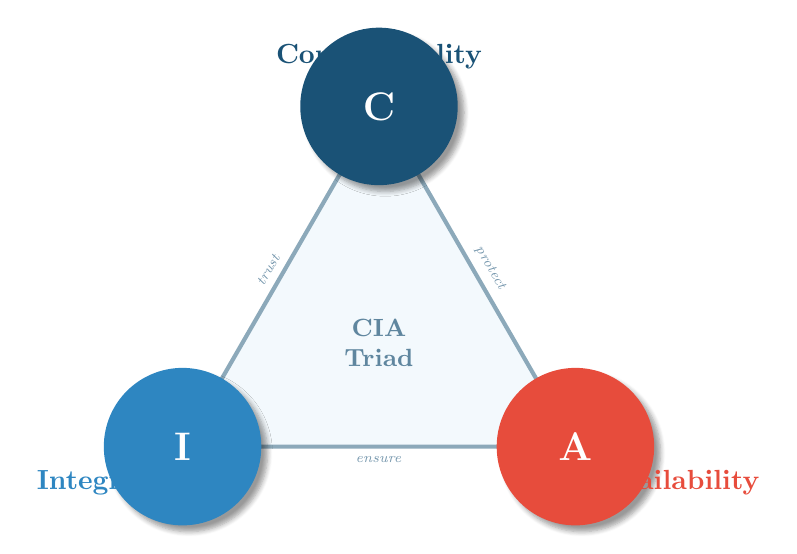
\begin{tikzpicture}[scale=1.2,
  circ/.style={circle, text=white, minimum size=2cm, font=\Large\bfseries,
    blur shadow={shadow blur steps=6, shadow xshift=0.8mm, shadow yshift=-0.8mm}}
]
  \coordinate (C) at (90:2.4);
  \coordinate (I) at (210:2.4);
  \coordinate (A) at (330:2.4);
  
  % Triangle fill
  \fill[lightbg, opacity=0.6] (C) -- (I) -- (A) -- cycle;
  \draw[very thick, primary!50, line width=1.5pt] (C) -- (I) -- (A) -- cycle;
  
  % Edge labels
  \node[font=\tiny, primary!60, rotate=60, above] at ($(C)!0.5!(I)$) {\textit{trust}};
  \node[font=\tiny, primary!60, rotate=-60, above] at ($(C)!0.5!(A)$) {\textit{protect}};
  \node[font=\tiny, primary!60, below] at ($(I)!0.5!(A)$) {\textit{ensure}};
  
  % Nodes
  \node[circ, fill=primary] at (C) {C};
  \node[circ, fill=secondary] at (I) {I};
  \node[circ, fill=accent] at (A) {A};
  
  % Labels
  \node[font=\bfseries, primary, above=0.35cm] at (C) {Confidentiality};
  \node[font=\bfseries, secondary, below left=0.25cm] at (I) {Integrity};
  \node[font=\bfseries, accent, below right=0.25cm] at (A) {Availability};
  
  % Center
  \node[font=\small\bfseries, primary!70, align=center] at (0,-0.1) {CIA\\Triad};
\end{tikzpicture}
\end{center}

\begin{definitionbox}[Confidentiality]
Ensuring that information is accessible only to those authorized to access it. Prevents unauthorized disclosure of data.\\
\textbf{Example:} Encryption, access control lists, authentication.
\end{definitionbox}

\begin{definitionbox}[Integrity]
Ensuring that information is accurate, complete, and has not been tampered with by unauthorized parties.\\
\textbf{Example:} Hashing (SHA-256), digital signatures, checksums.
\end{definitionbox}

\begin{definitionbox}[Availability]
Ensuring that information and resources are accessible to authorized users when needed.\\
\textbf{Example:} Redundancy, backups, load balancing, disaster recovery.
\end{definitionbox}

\subsection{Extended Security Properties}
\begin{itemize}[leftmargin=*]
  \item \textbf{Authentication:} Verifying the identity of a user, device, or system.
  \item \textbf{Authorization:} Determining what an authenticated user is permitted to do.
  \item \textbf{Non-repudiation:} Ensuring that a party cannot deny having performed an action (e.g., sending a message).
  \item \textbf{Accountability:} The ability to trace actions back to the responsible entity via logging and auditing.
\end{itemize}

%=============================================================
\section{Key Security Terminology}
%=============================================================

\rowcolors{2}{white}{defbg}
\begin{longtable}{@{}p{3.5cm}p{10cm}@{}}
\toprule
\rowcolor{primary!15}
\textbf{Term} & \textbf{Definition} \\
\midrule
\endhead
Asset & Anything of value (data, hardware, software, personnel). \\
\addlinespace
Threat & A potential cause of an unwanted incident that may harm an asset. \\
\addlinespace
Vulnerability & A weakness in a system that can be exploited by a threat. \\
\addlinespace
Exploit & A technique or tool used to take advantage of a vulnerability. \\
\addlinespace
Risk & The probability that a threat will exploit a vulnerability and cause harm. $\text{Risk} = \text{Threat} \times \text{Vulnerability} \times \text{Impact}$ \\
\addlinespace
Attack Surface & The total set of points where an attacker can try to enter or extract data. \\
\addlinespace
Threat Actor & An individual or group responsible for a cyber attack (hacker, insider, nation-state). \\
\addlinespace
Zero-Day & A vulnerability unknown to the vendor with no available patch. \\
\addlinespace
Patch & A software update that fixes a known vulnerability. \\
\addlinespace
Payload & The malicious code delivered by an exploit. \\
\addlinespace
Vector & The path or method used by an attacker to gain access. \\
\bottomrule
\end{longtable}

%=============================================================
\section{Security Models and Frameworks}
%=============================================================

\subsection{Defense in Depth}

A layered security strategy where multiple defenses are placed throughout the system.

\begin{center}
\begin{tikzpicture}[scale=0.9]
  \foreach \i/\lbl/\clr in {
    6/{\faIcon{building}~Physical Security}/red!18,
    5/{\faIcon{fire-alt}~Perimeter Security (Firewalls)}/orange!18,
    4/{\faIcon{network-wired}~Network Security (IDS/IPS)}/yellow!18,
    3/{\faIcon{desktop}~Host Security (Antivirus, Hardening)}/green!18,
    2/{\faIcon{code}~Application Security (Input Validation)}/blue!12,
    1/{\faIcon{database}~Data Security (Encryption)}/purple!12
  }{
    \pgfmathsetmacro{\w}{3.0+\i*1.2}
    \pgfmathsetmacro{\h}{0.75}
    \pgfmathsetmacro{\y}{(\i-1)*-1.05}
    \fill[\clr, rounded corners=3pt] (-\w/2, \y-\h/2) rectangle (\w/2, \y+\h/2);
    \draw[thick, black!40, rounded corners=3pt] (-\w/2, \y-\h/2) rectangle (\w/2, \y+\h/2);
    \node[font=\small\bfseries] at (0, \y) {\lbl};
  }
  % Vertical arrow
  \draw[-{Stealth}, very thick, primary!60, line width=2pt] (5.8,0.3) -- (5.8,-5.5)
    node[midway, right, font=\footnotesize\bfseries, primary!70, align=left] {Outer\\$\downarrow$\\Inner};
  \node[font=\footnotesize\itshape, primary!60, right] at (5.0, 0.7) {Layers of Defense};
\end{tikzpicture}
\end{center}

\subsection{The Principle of Least Privilege}
Users and programs should be granted only the minimum permissions needed to perform their tasks.

\subsection{Zero Trust Model}
\begin{conceptbox}[Zero Trust]
``Never trust, always verify.'' Every access request is fully authenticated, authorized, and encrypted---regardless of whether it originates inside or outside the network perimeter.
\end{conceptbox}

\subsection{AAA Framework}
\begin{itemize}[leftmargin=*]
  \item \textbf{Authentication:} Who are you? (passwords, biometrics, tokens)
  \item \textbf{Authorization:} What can you do? (permissions, roles)
  \item \textbf{Accounting:} What did you do? (logging, auditing)
\end{itemize}

%=============================================================
\section{Cryptography Fundamentals}
%=============================================================

\begin{definitionbox}[Cryptography]
The science of securing communication and data through encoding so that only intended recipients can read it.
\end{definitionbox}

\subsection{Types of Encryption}

\begin{center}
\begin{tikzpicture}[scale=0.82, transform shape,
  box/.style={rectangle, draw, thick, fill=#1, minimum width=2.4cm, minimum height=0.9cm, align=center, font=\small\bfseries, rounded corners=2pt},
  arr/.style={-{Stealth}, thick, primary!70}
]
  % --- Symmetric row ---
  \node[font=\bfseries, primary] at (2, 1.5) {Symmetric Encryption (e.g., AES, DES)};
  \node[box=green!15] (pt1) at (-4.5,0) {Plaintext};
  \node[box=yellow!20] (enc1) at (-1.2,0) {\faIcon{lock}~Encrypt};
  \node[box=red!15] (ct1) at (2.2,0) {Ciphertext};
  \node[box=yellow!20] (dec1) at (5.6,0) {\faIcon{unlock}~Decrypt};
  \node[box=green!15] (pt2) at (9,0) {Plaintext};
  
  \draw[arr] (pt1) -- (enc1);
  \draw[arr] (enc1) -- (ct1);
  \draw[arr] (ct1) -- (dec1);
  \draw[arr] (dec1) -- (pt2);
  
  % Key annotation
  \node[font=\small\bfseries, secondary, fill=blue!8, rounded corners=2pt, inner sep=3pt] at (2.2, -1.3) {\faIcon{key}~Same Secret Key};
  \draw[-{Stealth}, secondary, dashed, thick] (-1.2,-0.55) -- (-1.2,-1.3) -- (5.6,-1.3) -- (5.6,-0.55);
  
  % --- Asymmetric row ---
  \node[font=\bfseries, primary] at (2, -3) {Asymmetric Encryption (e.g., RSA, ECC)};
  \node[box=green!15] (pt3) at (-4.5,-4.5) {Plaintext};
  \node[box=cyan!15] (enc2) at (-1.2,-4.5) {\faIcon{lock}~Encrypt};
  \node[box=red!15] (ct2) at (2.2,-4.5) {Ciphertext};
  \node[box=cyan!15] (dec2) at (5.6,-4.5) {\faIcon{unlock}~Decrypt};
  \node[box=green!15] (pt4) at (9,-4.5) {Plaintext};
  
  \draw[arr] (pt3) -- (enc2);
  \draw[arr] (enc2) -- (ct2);
  \draw[arr] (ct2) -- (dec2);
  \draw[arr] (dec2) -- (pt4);
  
  % Two keys
  \node[font=\small\bfseries, greenhl!80!black, fill=green!8, rounded corners=2pt, inner sep=3pt] at (-1.2, -5.7) {\faIcon{key}~Public Key};
  \draw[-{Stealth}, greenhl!70!black, dashed, thick] (-1.2,-5.0) -- (-1.2,-5.5);
  \node[font=\small\bfseries, accent, fill=red!8, rounded corners=2pt, inner sep=3pt] at (5.6, -5.7) {\faIcon{key}~Private Key};
  \draw[-{Stealth}, accent, dashed, thick] (5.6,-5.0) -- (5.6,-5.5);
\end{tikzpicture}
\end{center}
\medskip

\begin{center}
\begin{tabular}{@{}p{6.5cm}p{6.5cm}@{}}
\toprule
\textbf{Symmetric Encryption} & \textbf{Asymmetric Encryption} \\
\midrule
Same key for encryption \& decryption & Two keys: public key \& private key \\
Faster & Slower but more secure for key exchange \\
Key distribution is a challenge & Public key can be shared openly \\
Examples: AES, DES, 3DES, Blowfish & Examples: RSA, ECC, Diffie-Hellman \\
\bottomrule
\end{tabular}
\end{center}

\subsection{Hashing}
\begin{definitionbox}[Hash Function]
A one-way function that converts input into a fixed-length output (digest). Used for integrity verification, \emph{not} encryption.\\
\textbf{Examples:} MD5 (deprecated), SHA-1 (deprecated), SHA-256, SHA-3.
\end{definitionbox}

\subsection{Digital Signatures and Certificates}
\begin{itemize}[leftmargin=*]
  \item \textbf{Digital Signature:} Uses the sender's private key to sign a message; recipient verifies with sender's public key. Provides authentication, integrity, and non-repudiation.
  \item \textbf{Digital Certificate:} An electronic document issued by a Certificate Authority (CA) binding a public key to an identity.
  \item \textbf{PKI (Public Key Infrastructure):} The framework of policies, hardware, software, and procedures for managing digital certificates.
\end{itemize}

%=============================================================
\section{Authentication Mechanisms}
%=============================================================

\subsection{Authentication Factors}
\begin{enumerate}[leftmargin=*]
  \item \textbf{Something you know} --- Password, PIN, security question.
  \item \textbf{Something you have} --- Smart card, security token, phone (OTP).
  \item \textbf{Something you are} --- Fingerprint, retina scan, facial recognition.
\end{enumerate}

\begin{definitionbox}[Multi-Factor Authentication (MFA)]
Using two or more authentication factors to verify identity. Significantly reduces the risk of unauthorized access.
\end{definitionbox}

\subsection{Password Security Best Practices}
\begin{itemize}[leftmargin=*]
  \item Use long, complex passwords (12+ characters)
  \item Use a password manager
  \item Never reuse passwords across services
  \item Enable MFA wherever possible
  \item Avoid dictionary words; use passphrases
\end{itemize}

%=============================================================
\section{Network Security Fundamentals}
%=============================================================

\subsection{The OSI Model and Security at Each Layer}

\begin{center}
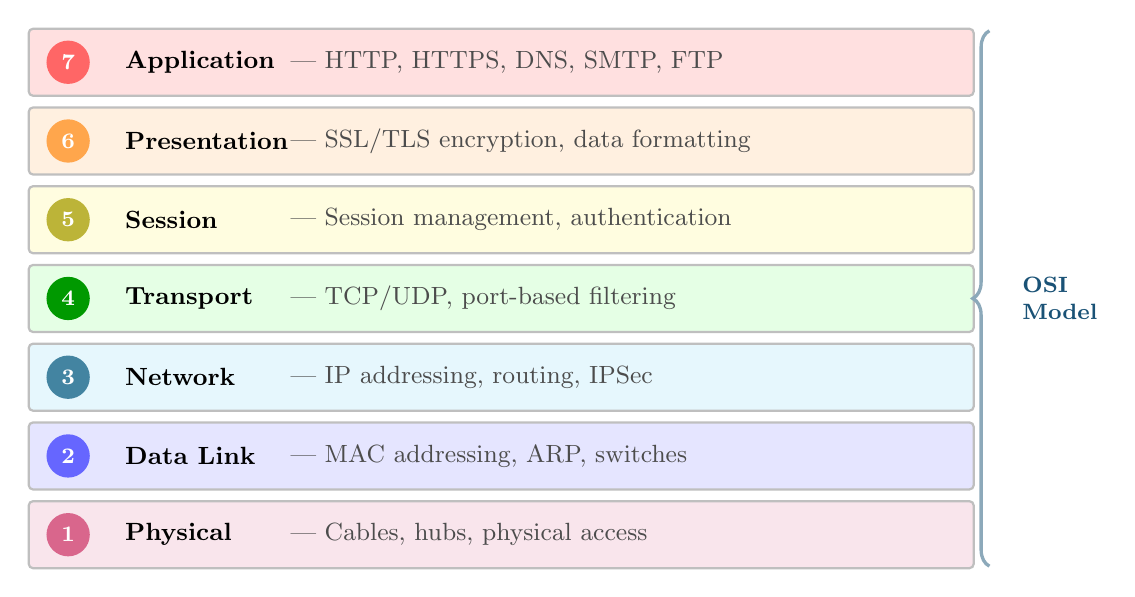
\begin{tikzpicture}[
  layer/.style={rectangle, draw, black!25, thick, fill=#1, minimum width=12cm, minimum height=0.85cm, font=\small, rounded corners=1.5pt},
  num/.style={circle, fill=#1, text=white, font=\footnotesize\bfseries, minimum size=0.55cm, inner sep=0pt}
]
  % Layer 7
  \node[layer=red!12] at (0, 0) {};
  \node[num=red!60] at (-5.5, 0) {7};
  \node[font=\small\bfseries, anchor=west] at (-4.9, 0) {Application};
  \node[font=\small, anchor=west, text=black!70] at (-2.8, 0) {--- HTTP, HTTPS, DNS, SMTP, FTP};
  % Layer 6
  \node[layer=orange!12] at (0,-1) {};
  \node[num=orange!70] at (-5.5,-1) {6};
  \node[font=\small\bfseries, anchor=west] at (-4.9,-1) {Presentation};
  \node[font=\small, anchor=west, text=black!70] at (-2.8,-1) {--- SSL/TLS encryption, data formatting};
  % Layer 5
  \node[layer=yellow!12] at (0,-2) {};
  \node[num=yellow!70!black] at (-5.5,-2) {5};
  \node[font=\small\bfseries, anchor=west] at (-4.9,-2) {Session};
  \node[font=\small, anchor=west, text=black!70] at (-2.8,-2) {--- Session management, authentication};
  % Layer 4
  \node[layer=green!10] at (0,-3) {};
  \node[num=green!60!black] at (-5.5,-3) {4};
  \node[font=\small\bfseries, anchor=west] at (-4.9,-3) {Transport};
  \node[font=\small, anchor=west, text=black!70] at (-2.8,-3) {--- TCP/UDP, port-based filtering};
  % Layer 3
  \node[layer=cyan!10] at (0,-4) {};
  \node[num=cyan!60!black] at (-5.5,-4) {3};
  \node[font=\small\bfseries, anchor=west] at (-4.9,-4) {Network};
  \node[font=\small, anchor=west, text=black!70] at (-2.8,-4) {--- IP addressing, routing, IPSec};
  % Layer 2
  \node[layer=blue!10] at (0,-5) {};
  \node[num=blue!60] at (-5.5,-5) {2};
  \node[font=\small\bfseries, anchor=west] at (-4.9,-5) {Data Link};
  \node[font=\small, anchor=west, text=black!70] at (-2.8,-5) {--- MAC addressing, ARP, switches};
  % Layer 1
  \node[layer=purple!10] at (0,-6) {};
  \node[num=purple!60] at (-5.5,-6) {1};
  \node[font=\small\bfseries, anchor=west] at (-4.9,-6) {Physical};
  \node[font=\small, anchor=west, text=black!70] at (-2.8,-6) {--- Cables, hubs, physical access};
  % Bracket
  \draw[decorate, decoration={brace, amplitude=6pt, mirror}, very thick, primary!50]
    (6.2,0.4) -- (6.2,-6.4) node[midway, right=8pt, font=\footnotesize\bfseries, primary, align=left] {OSI\\Model};
\end{tikzpicture}
\end{center}

\subsection{Key Network Security Devices and Technologies}

\begin{definitionbox}[Firewall]
A device or software that monitors and filters incoming and outgoing network traffic based on predefined security rules. Types: packet-filtering, stateful inspection, application-layer (WAF), next-generation (NGFW).
\end{definitionbox}

\begin{definitionbox}[Intrusion Detection System (IDS)]
Monitors network traffic for suspicious activity and generates alerts. It is \emph{passive}---it detects but does not block.
\end{definitionbox}

\begin{definitionbox}[Intrusion Prevention System (IPS)]
Similar to IDS but \emph{active}---it can automatically block or prevent detected threats.
\end{definitionbox}

\begin{definitionbox}[VPN (Virtual Private Network)]
Creates an encrypted tunnel over a public network (internet) to securely connect remote users or sites. Protocols: IPSec, OpenVPN, WireGuard.
\end{definitionbox}

\begin{definitionbox}[DMZ (Demilitarized Zone)]
A network segment that sits between the internal network and the internet, hosting public-facing servers while isolating them from the internal network.
\end{definitionbox}

\begin{definitionbox}[Proxy Server]
An intermediary server that forwards requests between clients and servers. Provides anonymity, caching, and content filtering.
\end{definitionbox}

\subsection{Network Security Architecture}

\begin{center}
\begin{tikzpicture}[
  box/.style={rectangle, draw, thick, fill=#1, minimum width=2.3cm, minimum height=1.1cm, align=center, font=\footnotesize\bfseries, rounded corners=4pt,
    blur shadow={shadow blur steps=5, shadow xshift=0.5mm, shadow yshift=-0.5mm}},
  arr/.style={{Stealth}-{Stealth}, thick, primary!60}
]
  \node[box=red!12] (inet) at (0,0) {\faIcon{globe}\\Internet};
  \node[box=orange!18] (fw1) at (3.2,0) {\faIcon{fire-alt}\\Outer\\Firewall};
  \node[box=yellow!15] (dmz) at (6.4,0) {\faIcon{server}\\DMZ\\(Web/Mail)};
  \node[box=orange!18] (fw2) at (9.6,0) {\faIcon{fire-alt}\\Inner\\Firewall};
  \node[box=green!12] (lan) at (12.8,0) {\faIcon{laptop}\\Internal\\LAN};
  
  \draw[arr] (inet) -- (fw1);
  \draw[arr] (fw1) -- (dmz);
  \draw[arr] (dmz) -- (fw2);
  \draw[arr] (fw2) -- (lan);
  
  \node[box=blue!12] (ids) at (6.4,-2.2) {\faIcon{eye}\\IDS/IPS\\Monitor};
  \draw[-{Stealth}, thick, dashed, secondary] (dmz) -- (ids);
  
  % Zone labels
  \node[font=\tiny\itshape, red!60!black, above=0.15cm] at (inet.north) {Untrusted};
  \node[font=\tiny\itshape, yellow!60!black, above=0.15cm] at (dmz.north) {Semi-Trusted};
  \node[font=\tiny\itshape, green!60!black, above=0.15cm] at (lan.north) {Trusted};
\end{tikzpicture}
\end{center}

\subsection{Wireless Network Security}
\begin{itemize}[leftmargin=*]
  \item \textbf{WEP (Wired Equivalent Privacy):} Deprecated; easily cracked.
  \item \textbf{WPA (Wi-Fi Protected Access):} Improved but still has weaknesses.
  \item \textbf{WPA2:} Uses AES encryption; current standard for most networks.
  \item \textbf{WPA3:} Latest standard with stronger encryption and protections against brute-force.
\end{itemize}

%=============================================================
\section{Common Cyber Attacks and Defenses}
%=============================================================

\begin{conceptbox}[Overview]
Attacks are categorized below by the layer or domain they target: \textbf{Human} (social engineering), \textbf{Network}, \textbf{Application}, \textbf{Endpoint} (malware), \textbf{Password}, and \textbf{Advanced/Emerging}. Each entry includes a definition and recommended defenses.
\end{conceptbox}

\subsection{Social Engineering Attacks (Human Layer)}

\begin{alertbox}[Phishing]
\textbf{Attack:} Fraudulent emails, messages, or websites designed to trick users into revealing sensitive information (passwords, credit card numbers).\\
\textbf{Defense:} Security awareness training, email filtering, verifying sender identity, anti-phishing tools.
\end{alertbox}

\begin{alertbox}[Spear Phishing]
\textbf{Attack:} A targeted phishing attack directed at a specific individual or organization using personalized information.\\
\textbf{Defense:} Employee training, verifying requests through alternate channels, email authentication (SPF, DKIM, DMARC).
\end{alertbox}

\begin{alertbox}[Social Engineering]
\textbf{Attack:} Manipulating people into divulging confidential information through pretexting, baiting, tailgating, or quid pro quo.\\
\textbf{Defense:} Security awareness programs, strict access policies, visitor management procedures.
\end{alertbox}

\begin{alertbox}[Shoulder Surfing]
\textbf{Attack:} Observing someone's screen or keyboard to steal information.\\
\textbf{Defense:} Privacy screens, awareness, shielding input when typing passwords.
\end{alertbox}

\begin{alertbox}[Dumpster Diving]
\textbf{Attack:} Searching through discarded materials (trash) to find sensitive information.\\
\textbf{Defense:} Shredding documents, secure disposal policies, encrypting discarded drives.
\end{alertbox}

\subsection{Network-Level Attacks}

\begin{alertbox}[Denial of Service (DoS)]
\textbf{Attack:} Overwhelming a system, server, or network with traffic to make it unavailable to legitimate users.\\
\textbf{Defense:} Rate limiting, traffic filtering, redundant infrastructure, content delivery networks (CDNs).
\end{alertbox}

\begin{alertbox}[Distributed Denial of Service (DDoS)]
\textbf{Attack:} A DoS attack launched from multiple compromised systems (botnet) simultaneously.\\
\textbf{Defense:} DDoS mitigation services (e.g., Cloudflare), traffic analysis, load balancing, ISP-level filtering.
\end{alertbox}

\begin{alertbox}[Man-in-the-Middle (MitM)]
\textbf{Attack:} The attacker secretly intercepts and possibly alters communication between two parties who believe they are communicating directly.\\
\textbf{Defense:} Use HTTPS/TLS, certificate pinning, VPNs, avoid public Wi-Fi for sensitive transactions.
\end{alertbox}

\begin{alertbox}[ARP Spoofing / ARP Poisoning]
\textbf{Attack:} Sending fake ARP messages to link the attacker's MAC address with a legitimate IP address, enabling traffic interception.\\
\textbf{Defense:} Static ARP entries, Dynamic ARP Inspection (DAI), network segmentation.
\end{alertbox}

\begin{alertbox}[DNS Spoofing / DNS Poisoning]
\textbf{Attack:} Corrupting the DNS cache to redirect users to malicious websites.\\
\textbf{Defense:} DNSSEC, secure DNS resolvers (DoH/DoT), regular cache flushing.
\end{alertbox}

\begin{alertbox}[IP Spoofing]
\textbf{Attack:} Forging the source IP address in packets to impersonate another system.\\
\textbf{Defense:} Ingress/egress filtering, packet authentication, IPSec.
\end{alertbox}

\begin{alertbox}[Packet Sniffing / Eavesdropping]
\textbf{Attack:} Capturing network packets to read unencrypted data (passwords, emails).\\
\textbf{Defense:} Encrypt traffic (TLS/SSL, VPN), use switched networks, network monitoring.
\end{alertbox}

\begin{alertbox}[Session Hijacking]
\textbf{Attack:} Stealing or predicting a valid session token to gain unauthorized access to a web application.\\
\textbf{Defense:} Use HTTPS, regenerate session IDs after login, set secure/HttpOnly cookie flags, session timeout.
\end{alertbox}

\subsection{Application-Level Attacks}

\begin{alertbox}[SQL Injection (SQLi)]
\textbf{Attack:} Inserting malicious SQL code into input fields to manipulate or access the database.\\
\textbf{Defense:} Parameterized queries (prepared statements), input validation, ORM frameworks, least privilege DB accounts.
\end{alertbox}

\begin{alertbox}[Cross-Site Scripting (XSS)]
\textbf{Attack:} Injecting malicious scripts into web pages viewed by other users to steal cookies, session tokens, or redirect users.\\
\textbf{Defense:} Output encoding, Content Security Policy (CSP), input sanitization, HttpOnly cookies.
\end{alertbox}

\begin{alertbox}[Cross-Site Request Forgery (CSRF)]
\textbf{Attack:} Tricking a logged-in user's browser into making an unwanted request to a web application.\\
\textbf{Defense:} Anti-CSRF tokens, SameSite cookie attribute, re-authentication for sensitive actions.
\end{alertbox}

\begin{alertbox}[Buffer Overflow]
\textbf{Attack:} Writing more data to a buffer than it can hold, causing adjacent memory to be overwritten, potentially allowing code execution.\\
\textbf{Defense:} Input validation, bounds checking, ASLR (Address Space Layout Randomization), DEP (Data Execution Prevention), safe coding practices.
\end{alertbox}

\begin{alertbox}[Remote Code Execution (RCE)]
\textbf{Attack:} Exploiting a vulnerability to execute arbitrary code on a remote system.\\
\textbf{Defense:} Regular patching, input validation, sandboxing, least privilege.
\end{alertbox}

\begin{alertbox}[Directory Traversal]
\textbf{Attack:} Exploiting insufficient input validation to access files outside the intended directory (e.g., using \texttt{../../etc/passwd}).\\
\textbf{Defense:} Input validation, chroot jails, restrict file system permissions.
\end{alertbox}

\subsection{Malware Attacks (Endpoint Level)}

\begin{alertbox}[Virus]
\textbf{Attack:} A malicious program that attaches itself to legitimate files and spreads when the host file is executed.\\
\textbf{Defense:} Antivirus software, avoid untrusted downloads, keep systems updated.
\end{alertbox}

\begin{alertbox}[Worm]
\textbf{Attack:} Self-replicating malware that spreads across networks without user interaction.\\
\textbf{Defense:} Firewalls, IDS/IPS, network segmentation, patch management.
\end{alertbox}

\begin{alertbox}[Trojan Horse]
\textbf{Attack:} Malware disguised as legitimate software that provides unauthorized access or performs malicious actions.\\
\textbf{Defense:} Download software from trusted sources, antivirus, application whitelisting.
\end{alertbox}

\begin{alertbox}[Ransomware]
\textbf{Attack:} Malware that encrypts the victim's files and demands a ransom payment for decryption.\\
\textbf{Defense:} Regular backups (offline/offsite), patch management, email filtering, endpoint detection and response (EDR).
\end{alertbox}

\begin{alertbox}[Spyware]
\textbf{Attack:} Software that secretly monitors user activity and collects personal information.\\
\textbf{Defense:} Anti-spyware tools, avoid suspicious downloads, regular scans.
\end{alertbox}

\begin{alertbox}[Rootkit]
\textbf{Attack:} Malware that hides its presence and provides continued privileged access to a system.\\
\textbf{Defense:} Integrity checking tools, secure boot, rootkit scanners, reinstallation if detected.
\end{alertbox}

\begin{alertbox}[Keylogger]
\textbf{Attack:} Software or hardware that records keystrokes to capture passwords and sensitive data.\\
\textbf{Defense:} Anti-keylogger software, virtual keyboards, MFA, endpoint protection.
\end{alertbox}

\begin{alertbox}[Botnet]
\textbf{Attack:} A network of compromised computers (bots/zombies) controlled by an attacker, often used for DDoS or spam.\\
\textbf{Defense:} Antivirus, firewalls, intrusion detection, regular patching, network monitoring.
\end{alertbox}

\subsection{Password Attacks}

\begin{alertbox}[Brute Force Attack]
\textbf{Attack:} Systematically trying every possible combination of characters to guess a password.\\
\textbf{Defense:} Account lockout policies, strong passwords, CAPTCHA, MFA, rate limiting.
\end{alertbox}

\begin{alertbox}[Dictionary Attack]
\textbf{Attack:} Using a list of common words and known passwords to guess credentials.\\
\textbf{Defense:} Complex passwords, avoid common words, salted hashing.
\end{alertbox}

\begin{alertbox}[Rainbow Table Attack]
\textbf{Attack:} Using precomputed hash-to-password lookup tables to crack hashed passwords.\\
\textbf{Defense:} Use salted hashes, strong hashing algorithms (bcrypt, Argon2).
\end{alertbox}

\begin{alertbox}[Credential Stuffing]
\textbf{Attack:} Using stolen username/password pairs from data breaches to access other services.\\
\textbf{Defense:} Unique passwords per service, MFA, breach monitoring.
\end{alertbox}

\subsection{Advanced / Emerging Attacks}

\begin{alertbox}[Advanced Persistent Threat (APT)]
\textbf{Attack:} A prolonged, targeted cyber attack where an intruder gains access and remains undetected for an extended period.\\
\textbf{Defense:} Network monitoring, threat intelligence, segmentation, incident response planning, EDR.
\end{alertbox}

\begin{alertbox}[Zero-Day Exploit]
\textbf{Attack:} Exploiting a previously unknown vulnerability before a patch is available.\\
\textbf{Defense:} Behavioral detection, sandboxing, threat intelligence, rapid patch deployment.
\end{alertbox}

\begin{alertbox}[Supply Chain Attack]
\textbf{Attack:} Compromising a trusted third-party vendor or software update mechanism to distribute malware.\\
\textbf{Defense:} Vendor assessment, code signing verification, software bill of materials (SBOM), integrity checks.
\end{alertbox}

\begin{alertbox}[Insider Threat]
\textbf{Attack:} A current or former employee, contractor, or business associate who misuses authorized access to harm the organization.\\
\textbf{Defense:} Least privilege, user activity monitoring, background checks, separation of duties.
\end{alertbox}

%=============================================================
\section{Summary: Attacks and Defenses at a Glance}
%=============================================================

\begin{center}
\small
\rowcolors{2}{white}{lightbg}
\begin{longtable}{@{}p{2.8cm}p{3.5cm}p{2.5cm}p{4.5cm}@{}}
\toprule
\rowcolor{primary!15}
\textbf{Layer} & \textbf{Attack} & \textbf{Target} & \textbf{Key Defense} \\
\midrule
\endhead
Human & Phishing & Users & Training, email filters \\
Human & Social Engineering & Users & Awareness, policies \\
\addlinespace
Network & DoS/DDoS & Servers & Rate limiting, CDN, filtering \\
Network & MitM & Communication & TLS, VPN, cert pinning \\
Network & ARP Spoofing & LAN & DAI, static ARP \\
Network & DNS Spoofing & DNS & DNSSEC, secure resolvers \\
Network & Sniffing & Traffic & Encryption, VPN \\
\addlinespace
Application & SQL Injection & Database & Parameterized queries \\
Application & XSS & Web users & CSP, output encoding \\
Application & CSRF & Web sessions & Anti-CSRF tokens \\
Application & Buffer Overflow & Memory & ASLR, DEP, bounds check \\
\addlinespace
Endpoint & Ransomware & Files & Backups, EDR, patching \\
Endpoint & Virus/Worm & Systems & Antivirus, segmentation \\
Endpoint & Rootkit & OS & Integrity checks, secure boot \\
\addlinespace
Password & Brute Force & Credentials & Lockout, MFA, rate limit \\
Password & Rainbow Table & Hashes & Salted hashing \\
\addlinespace
Advanced & APT & Organization & Monitoring, threat intel \\
Advanced & Zero-Day & Any & Behavioral detection \\
Advanced & Supply Chain & Software & Code signing, SBOM \\
\bottomrule
\end{longtable}
\end{center}

%=============================================================
\section{Security Best Practices Checklist}
%=============================================================

\begin{multicols}{2}
\begin{itemize}[leftmargin=1.5em, itemsep=2pt]
  \item[{\textcolor{greenhl}{\faIcon{check-circle}}}] Keep all software updated and patched
  \item[{\textcolor{greenhl}{\faIcon{check-circle}}}] Use strong, unique passwords with MFA
  \item[{\textcolor{greenhl}{\faIcon{check-circle}}}] Encrypt sensitive data at rest and in transit
  \item[{\textcolor{greenhl}{\faIcon{check-circle}}}] Implement the principle of least privilege
  \item[{\textcolor{greenhl}{\faIcon{check-circle}}}] Conduct regular security awareness training
  \item[{\textcolor{greenhl}{\faIcon{check-circle}}}] Perform regular backups (3-2-1 rule)
  \item[{\textcolor{greenhl}{\faIcon{check-circle}}}] Deploy firewalls and IDS/IPS
  \item[{\textcolor{greenhl}{\faIcon{check-circle}}}] Segment networks appropriately
  \item[{\textcolor{greenhl}{\faIcon{check-circle}}}] Monitor and log all access and activities
  \item[{\textcolor{greenhl}{\faIcon{check-circle}}}] Have an incident response plan
  \item[{\textcolor{greenhl}{\faIcon{check-circle}}}] Conduct regular vulnerability assessments
  \item[{\textcolor{greenhl}{\faIcon{check-circle}}}] Implement endpoint protection
  \item[{\textcolor{greenhl}{\faIcon{check-circle}}}] Use secure coding practices
  \item[{\textcolor{greenhl}{\faIcon{check-circle}}}] Verify third-party software integrity
\end{itemize}
\end{multicols}

%=============================================================
\section{Incident Response Lifecycle}
%=============================================================

\begin{center}
\begin{tikzpicture}[
  phase/.style={rectangle, draw, thick, fill=#1, minimum width=2.6cm, minimum height=1.3cm, align=center, font=\small\bfseries, rounded corners=6pt,
    blur shadow={shadow blur steps=5, shadow xshift=0.5mm, shadow yshift=-0.5mm}},
  arr/.style={-{Stealth[length=3mm]}, very thick, primary!60, line width=1.5pt}
]
  % Circular layout
  \node[phase=blue!15]   (p1) at (90:3.2)  {\faIcon{clipboard-list}\\Preparation};
  \node[phase=orange!15] (p2) at (18:3.2)  {\faIcon{search}\\Detection \&\\Analysis};
  \node[phase=red!15]    (p3) at (-54:3.2) {\faIcon{ban}\\Containment \&\\Eradication};
  \node[phase=green!15]  (p4) at (-126:3.2){\faIcon{redo}\\Recovery};
  \node[phase=purple!15] (p5) at (-198:3.2){\faIcon{graduation-cap}\\Lessons\\Learned};
  
  \draw[arr] (p1) to[bend right=18] (p2);
  \draw[arr] (p2) to[bend right=18] (p3);
  \draw[arr] (p3) to[bend right=18] (p4);
  \draw[arr] (p4) to[bend right=18] (p5);
  \draw[arr] (p5) to[bend right=18] (p1);
  
  % Center label
  \node[font=\small\bfseries, primary!60, align=center] at (0,0) {Incident\\Response\\Lifecycle};
\end{tikzpicture}
\end{center}

\begin{enumerate}[leftmargin=*]
  \item \textbf{Preparation:} Establish policies, tools, and a response team.
  \item \textbf{Detection \& Analysis:} Identify and investigate security incidents.
  \item \textbf{Containment \& Eradication:} Isolate affected systems and remove the threat.
  \item \textbf{Recovery:} Restore systems to normal operations.
  \item \textbf{Lessons Learned:} Review the incident to improve future response.
\end{enumerate}

%=============================================================
\section{Review Questions}
%=============================================================

\begin{enumerate}[leftmargin=*]
  \item Define the CIA triad and give one example for each property.
  \item What is the difference between a vulnerability, a threat, and an exploit?
  \item Compare symmetric and asymmetric encryption with examples.
  \item Explain the difference between IDS and IPS.
  \item What is a Man-in-the-Middle attack and how can it be prevented?
  \item Describe three types of malware and their defenses.
  \item What is the principle of least privilege and why is it important?
  \item How does SQL injection work and what are the best defenses?
  \item Explain the Defense in Depth strategy with an example.
  \item What is multi-factor authentication and why is it recommended?
\end{enumerate}

\end{document}
